In questa sezione si riportano i preventivi per le varie fasi di lavoro elencate nel capitolo precedente. \newline
Si ricorda che il progetto didattico impone il vincolo che tutti i membri del gruppo ricoprino tutti i ruoli in modo equo.
Il gruppo rispetterà il vincolo nel progetto complessivo e non nelle singole fasi, 
altrimenti non si riuscirà a dare continuità al ruolo terminando i task assegnati.

\subsection{RTB}
\subsubsection{Baseline documentale}
\paragraph{Prospetto orario}
\begin{center}
	\renewcommand{\arraystretch}{1.8} %aumento ampiezza righe
	\begin{tabular}{ |m{10em}|c|c|c|c|c|c|c| }
	\hline
	\textbf{Membro} & \textbf{Re} & \textbf{Am} &  \textbf{An} &  \textbf{Pt} &  \textbf{Pg} &  \textbf{Ve} &  \textbf{Totale}\\
    \hline
    Irene Benetazzo   & 3 & - & 3 & - & - & - & \textbf{6} \\
    \hline
    Tommaso Berlaffa  & - & 5 & - & - & - & 1 & \textbf{6} \\
    \hline
    Mattia Episcopo   & - & 6 & - & - & - & - & \textbf{6} \\
    \hline
    Pietro Macrì      & - & 5 & - & - & - & 2 & \textbf{7} \\
    \hline
    Qi Fan Andrea Pan & - & 4 & 3 & - & - & - & \textbf{7} \\
    \hline
    Matteo Pillon     & - & 7 & - & - & - & - & \textbf{7} \\
    \hline
    Samuele Rizzato   & - & 4 & 3 & - & - & - & \textbf{7} \\
    \hline
    \textbf{Totale ore} & \textbf{3} & \textbf{31} &  \textbf{9} &  \textbf{0} &  \textbf{0} &  \textbf{3} &  \textbf{46}\\
    \hline
	\end{tabular}
\end{center}
\begin{figure}[H]
    \centering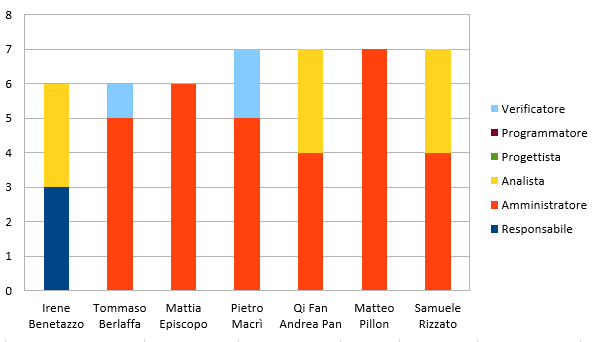
\includegraphics[width=\textwidth, height=\textheight, keepaspectratio]{images/preventivo/RTB-documentale-ore.png}
\end{figure}


\paragraph{Prospetto economico}
\begin{center}
	\renewcommand{\arraystretch}{1.8} %aumento ampiezza righe
	\begin{tabular}{ |m{10em}|c|c|c|c|c|c|c| }
	\hline
	\textbf{Ruolo} & \textbf{Re} & \textbf{Am} &  \textbf{An} &  \textbf{Pt} &  \textbf{Pg} &  \textbf{Ve} &  \textbf{Totale}\\
    \hline
    Totale ore & 3 & 31 & 9 & 0 & 0 & 3 & \textbf{46}\\
    \hline
    Costo \euro/h & 30\euro/h & 20\euro/h & 25\euro/h & 25\euro/h & 15\euro/h & 15\euro/h & \\
    \hline
    \textbf{Totale costo} & \textbf{90\euro} & \textbf{620\euro} &  \textbf{225\euro} &  \textbf{0\euro} &  \textbf{0\euro} &  \textbf{45\euro} &  \textbf{980\euro}\\
    \hline
	\end{tabular}

    \begin{figure}[H]
        \centering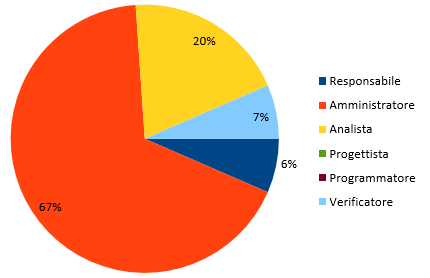
\includegraphics[width=0.7\textwidth, height=0.7\textheight, keepaspectratio]{images/preventivo/RTB-documentale-costo.png}
    \end{figure}
\end{center}


\subsubsection{Baseline dei requisiti}
\paragraph{Prospetto orario}
\begin{center}
	\renewcommand{\arraystretch}{1.8} %aumento ampiezza righe
	\begin{tabular}{ |m{10em}|c|c|c|c|c|c|c| }
	\hline
	\textbf{Membro} & \textbf{Re} & \textbf{Am} &  \textbf{An} &  \textbf{Pt} &  \textbf{Pg} &  \textbf{Ve} &  \textbf{Totale}\\
    \hline
    Irene Benetazzo   & - & 3 & 11 & - & - & 2 & \textbf{16} \\
    \hline
    Tommaso Berlaffa  & - & 1 & 13 & - & - & - & \textbf{14} \\
    \hline
    Mattia Episcopo   & - & 2 & 11 & - & - & - & \textbf{13} \\
    \hline
    Pietro Macrì      & - & 1 & 13 & - & - & - & \textbf{14} \\
    \hline
    Qi Fan Andrea Pan & - & 1 & 12 & - & - & - & \textbf{13} \\
    \hline
    Matteo Pillon     & - & 1 & 13 & - & - & 2 & \textbf{16} \\
    \hline
    Samuele Rizzato   & 3 & 1 & 11 & - & - & - & \textbf{15} \\
    \hline
    \textbf{Totale ore} & \textbf{3} & \textbf{10} &  \textbf{84} &  \textbf{0} &  \textbf{0} &  \textbf{4} &  \textbf{101}\\
    \hline
	\end{tabular}
\end{center}
\begin{figure}[H]
    \centering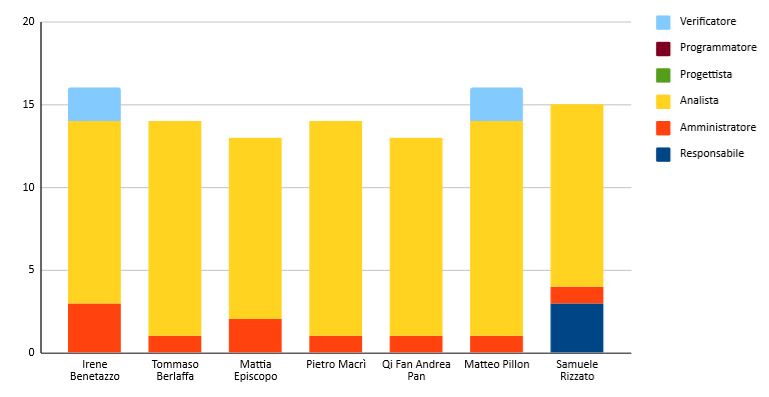
\includegraphics[width=\textwidth, height=\textheight,keepaspectratio]{images/preventivo/RTB-requisiti-ore.png}
\end{figure}

\paragraph{Prospetto economico}
\begin{center}
	\renewcommand{\arraystretch}{1.8} %aumento ampiezza righe
	\begin{tabular}{ |m{10em}|c|c|c|c|c|c|c| }
	\hline
	\textbf{Ruolo} & \textbf{Re} & \textbf{Am} &  \textbf{An} &  \textbf{Pt} &  \textbf{Pg} &  \textbf{Ve} &  \textbf{Totale}\\
    \hline
    Totale ore & 3 & 10 & 84 & 0 & 0 & 4 & \textbf{101}\\
    \hline
    Costo \euro/h & 30\euro/h & 20\euro/h & 25\euro/h & 25\euro/h & 15\euro/h & 15\euro/h & \\
    \hline
    \textbf{Totale costo} & \textbf{90\euro} & \textbf{200\euro} &  \textbf{2100\euro} &  \textbf{0\euro} &  \textbf{0\euro} &  \textbf{60\euro} &  \textbf{2450\euro}\\
    \hline
	\end{tabular}

    \begin{figure}[H]
        \centering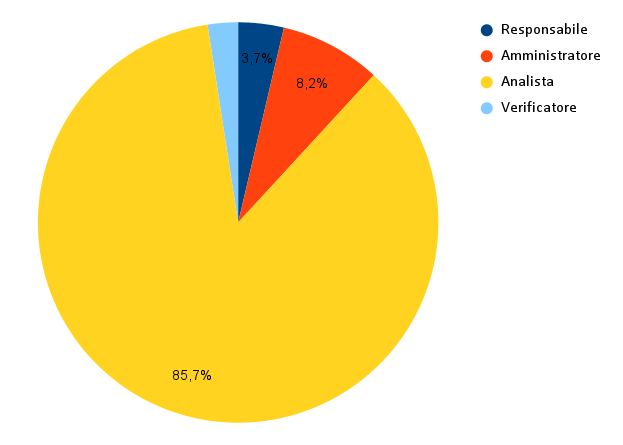
\includegraphics[width=0.7\textwidth, height=0.7\textheight, keepaspectratio]{images/preventivo/RTB-requisiti-costo.png}
    \end{figure}
    
\end{center}

\subsubsection{Baseline delle tecnologie}


\newpage